\newpage
\section{Esempi ed esercizi}

% aggiungere batch 1

\subsection{Campionamento}
$$x(n) = A\cos(\omega n + \theta)$$
\begin{figure}[h]
	\centering
	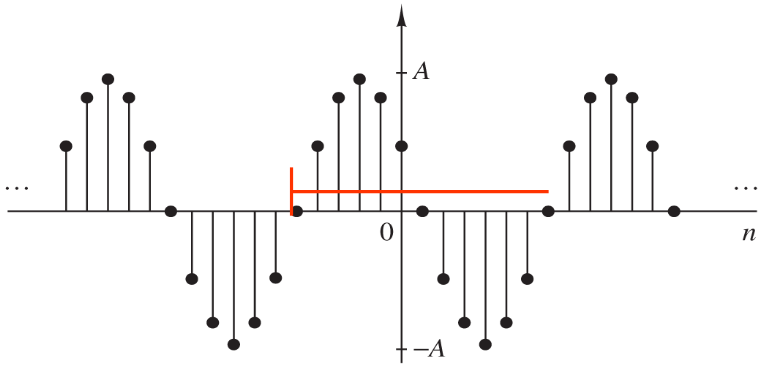
\includegraphics[scale=0.56]{Lezioni/Immagini/esempio1}
\end{figure}

$\omega = 2\pi f_N$, dove $\omega$ è la pulsazione e $f_N$ la frequenza normalizzata, cioè il numero di cicli al secondo (continuo), con campioni al posto dei secondi nel mondo campionato.

Per capire la frequenza $f_N$ del segnale rappresentato, bisogna guardare quanti cicli ci sono per campioni (o quanti campioni ci sono in un ciclo, cioè prima che il pattern si ripeta) e calcolare l'inverso. In questo caso un periodo è 12 campioni, quindi $f_N = 1/12$.

La frequenza al secondo (Hz) è ottenibile sapendo quanta distanza c'è tra un campione e l'altro, altrimenti per ogni rappresentazione ci sarebbero infinite sinusoidi.

La pulsazione $\omega$ è uguale a $2\pi f_N$, quindi $\frac{2\pi}{12} = \frac{\pi}{6}$. \\
Lo sfasamento con anticipo di 2 campioni si trova effettuando la proporzione: un periodo è $2\pi$, se 12 campioni sono in$2\pi$ allora $2\pi : 12 = \theta : 2 \rightarrow \theta = \frac{\pi}{3}$.

La frequenza normalizzata indica quanto bene si vedono i campioni e la loro variazione in un periodo, per poi decidere la finestra di osservazione. La frequenza dipende dal numero di campioni al secondo ($f_c$): se la frequenza di campionamento è $f_c = 1$ campione/secondo, si ha che $f = 1/12$ ciclo/secondo, cioè $f = f_c \cdot f_N$.

Per ricavare la formula più facilmente si possono utilizzare le unità di misura. Un altro modo per arrivare allo stesso risultato è sostituire a $n\Delta t$ la $t$.
\newpage
Con 2 campioni al secondo, cioè $f_c = 2$ e $\Delta t = 0.5 = \nicefrac{1}{2}$, la frequenza $f$ in cicli al secondo (Hz) è $\nicefrac{1}{2}$:
$$f_N \cdot f_c = \frac{1}{12} \frac{\text{cicli}}{\text{campione}} \cdot \frac{2 \text{ campioni}}{\text{sec}} = \frac{1}{6} \frac{\text{cicli}}{\text{sec}}$$
$$x(n) = A\cos \Big(2\pi \frac{1}{12}n + \frac{\pi}{3}\Big) \implies x(t) = A\cos\Big(2\pi \frac{1}{6}t + \frac{\pi}{3}\Big) \qquad \Delta tn \implies t$$

\subsection{Convoluzione}
Per rappresentare una convoluzione è necessario conoscere la posizione dello 0 sull'asse $x$, e rappresentare sia i campioni di $h(m)$ che di $f(m)$. Si ricorda che $\Delta m$ esiste solo quando l'argomento si annulla.

Il segnale $h(m)$ viene traslato e ribaltato rispetto all'asse $x$ con $n = -\infty, \dots, +\infty$ (anche se la proprietà è commutativa quindi il risultato sarebbe identico utilizzando $f(m)$. 

$y(n)$ è la funzione che si ottiene quando il segnale ottenuto assume valore $n$. \\
Si ha $y(n) = \sum_{-\infty}^{max+\infty} x(m)h(n - m)$.

% finire

\subsection{Quantizzazione}
\subsubsection{}
Dato il segnale a tempo discreto $x(n) = 6,4 \cos (\nicefrac{\pi}{10}n)$, trovare il numero (intero) di bit necessari per la conversione da analogico a digitale tale che:
\begin{enumerate}
	\item $\Delta = 0,1$: \\
	$0,1 \cdot 2^b \geq 12,8 \rightarrow 2^b \geq \frac{12,8}{0,1} = 128 \rightarrow b = 7$ \\
	$SNR_q = 1,76 + 6,02b = 43,9 dB$
	\item $\Delta = 0,02$: \\
	$0,02 \cdot 2^b \geq 12,8 \rightarrow 2^b \geq \frac{128}{0,02} = 640 \rightarrow b = 9 \lor 10$ \\
	$2^9 = 540 \qquad 2^10= 1024$ \\
	Il valore scelto dev'essere sempre il maggiore (10) altrimenti si verifica saturazione. Il numero perfetto sarebbe una potenza che soddisfa esattamente l'equazione $D_S = D_q$, ma non sempre è possibile averne uno. \\
	$SNR_q = 1,76 + 6,02b = 61,96 dB$ se fosse ottimale;
	$SNR_q = 10\log_{10} \frac{(6,4)^2}{0,02 / 12} = 57,88 dB$ nel caso vero.
	\end{enumerate}

Bisogna sempre rispettare $D_s \leq D_q$, pertanto $D_s = 2 \cdot 6,4 = 12,8$. La dinamica del quantizzatore è $\Delta 2^b$. 

Il rapporto segnale-rumore ($SNR_q$) del secondo caso è minore di quello ideale, ma comunque maggiore del primo, quindi la seconda $\Delta$ è più efficiente.

\subsubsection{}
Con $b = 10$, $2A = 12,8$, trovare la $\Delta$ tale che il rapporto segnale-rumore sia ottimo. Sapendo che la frequenza massima è $15 kHz$ ma la frequenza campionata è $27 kHz$, calcolare il rapporto segnale-rumore.

$Dq = Ds \rightarrow \Delta = \frac{12,8}{1024} = 0,0125$

Se la frequenza massima è $15 kHz$, la densità spettrale (potenza) uniforme è $P = \abs{F(\delta(x))}$. \\
Il range in kHz è $[-15, +15]$ e ha una distribuzione uniforme, quindi sarà rappresentato con una finestra. 
Se la frequenza di campionamento è minore di 30, ci saranno fenomeni di aliasing e sotto-campionamento. 

Con $f_c = 27 kHz$, la finestra occupata sarà $[-13,5,\: 13,5]$ e la replica si posizionerà nella fascia non utilizzata in modo simmetrico rispetto all'estremo dell'intervallo. Le frequenze più alte verranno erroneamente convertite in frequenze basse.

La replica si posiziona a $-15 kkHz + 27kHz = 12 kHz$. \\
Di conseguenza, la parte corretta sarà $[-12, +12]$.

Non è possibile trovare il rumore delle frequenze che si sovrappongono da $12 kHz$ a $13,5 kHz$ perché è parte integrante del segnale.

Rapporto segnale-distorsione: applicando la definizione di rapporto segnale-rumore, è possibile calcolare l'integrale. \\
Si ha $S$ come periodo che va da $-\nicefrac{f_c}{2}$ a $\nicefrac{f_c}{2}$, quindi:
$$S = \int_{-f_c/2}^{f_c/2}\abs{x(f)}^2ndf \quad \implies \quad S = 2\int_{0}^{13,5} df = 27u$$

$$D = \int_{f_c/2}^{\infty} \abs{x(h)}^2 df +  \int_{-\infty}^{f_c/2}\abs{x(f)}^2ndf \quad \implies \quad D = 2\int_{-\infty}^{-13,5} df = 2\int_{13,5}^{15} df = 3u$$

$$SNR_c = 10\log_{10} \frac{P_S = S}{P_R = D} = \frac{27u}{3u} = 9,54 dB$$

\subsection{Frequenze}
\subsubsection{}
Due segnali analogici, $x(t) = 5\sin(60\pi t)$ e $y(t) = 2\cos(60\pi t) - 3\sin(40\pi t)$, vengono sommati e campionati con una frequenza di campionamento $f_c = 50 Hz$. 
\begin{enumerate}
	\item Rappresentare graficamente i due segnali sommati;
	\item Rappresentare il segnale con aliasing;
	\item Caratterizzare ($\Delta$, numero di bit) un quantizzatore ideale per il segnale, in modo che il rapporto segnale-rumore sia circa $96 dB$;
	\item Trovare la frequenza normalizzata.
\end{enumerate}
La somma di funzioni è:
$$z(t) = 5\sin(60\pi t) + 2\cos(60\pi t) - 3\sin(40\pi t)$$
Seno e coseno non hanno distinzione nella trasformata, quindi è necessario rappresentare la parte reale (coseno) e la parte immaginaria (seno). 

Un seno può quindi essere confuso al più con un altro seno avente frequenze minori, mai con un coseno.

$60\pi t = 2\pi 30t$ \\
La parte reale avrà due picchi a $[-30, +30]$ alti 1 ($\nicefrac{2}{2}$), mentre la parte immaginaria avrà gli stessi, alti $\nicefrac{5}{2}$, uno positivo e uno negativo. 30 cicli al secondo sono $30Hz$.

Lo stesso procedimento si applica al seno, per ottenere il segnale prima del campionamento. C'è aliasing, perché $50 < 2 \cdot 30$. 

Il primo picco nella parte reale trasla fino a $+20$, e il secondo esce dall'intervallo. Il periodo base è largo $50 Hz$, e va osservato centrato in 0 con un'ampiezza di $[-25, +25]$. La seconda replica va da 30 a $(30 - 50)$, cioè $-20$. La parte immaginaria ha un range $[-25, +\infty]$.

Il segnale frainteso con aliasing diventa:
$$z'(t) = 2\cos(40\pi t) - 8\sin(40\pi t)$$
Se il segnale ha un range maggiore del quantizzatore ideale, per esempio ottenuto sommando più sinusoidali, esso satura.

Per avere un rapporto segnale-rumore di $96 db$, si ha che $SNR_Q = 1,76 + 6,02b \approx 96db$. \\
Di conseguenza $b = 16$, $\Delta = \frac{10}{2^b}$ ma il segnale satura a causa dell'aliasing.

La frequenza normalizzata è $F_N = \frac{\text{cicli}}{\text{campione}} = \frac{F}{f_c}$ (dove $F$ è il coefficiente che moltiplica $2\pi t$), cioè rispettivamente $\nicefrac{3}{5}$, $\nicefrac{3}{5}$ e $\nicefrac{2}{5}$ per le sinusoidali. I primi due valori, però, non sono nell'intervallo $[-1/2, +1/2]$ (frequenza di Nyquist) quindi va sottratto 1. 

Se il coseno ha un coefficiente negativo, bisogna ricordare che la funzione è pari, quindi ha lo stesso aspetto a prescindere dal segno.

La nuova funzione normalizzata è:
$$z(t) = -5\sin\Big(2\pi \frac{2}{5}n\Big) + 2\cos\Big(2\pi \frac{2}{5}n\Big) - 3\sin\Big(2\pi \frac{2}{5}n\Big)$$
Le due funzioni seno si possono semplificare scrivendo: 
$$z(t) = +2\cos\Big(2\pi \frac{2}{5}n\Big) - 8\sin\Big(2\pi \frac{2}{5}n\Big)$$
Bisogna notare che $n$ è al posto di $t$ avendo trasformato dal dominio del tempo a quello dei campioni. 

$f = \frac{2}{5} \frac{\text{cicli}}{\text{campione}} \cdot 50 \frac{\text{campioni}}{\text{secondo}} = 20 \frac{\text{cicli}}{\text{secondo}}$ \\
$\Delta t = \nicefrac{1}{f_c}$, con $F_N = 25Hz$ l'intervallo sarà $[-25, +25]$.

\subsection{Trasformate di Fourier}
\subsubsection{}

\subsection{Relazioni I/O}
% slide 11
Se non ci fosse il modulo, il segnale sarebbe una rampa: in questo caso ha una forma di V, a tempo discreto. 

1) è l'identità, 3*delta(n+3), 2*delta(n+2), 1*delta(n+1), ... mettendo a 0 l'argomento \\
2) segnale in ritardo (in anticipo non è possibile), uguale a sopra ma cambia l'origine \\
3) funzione mediana su 3 valori, in cui la mediana considera il valore centrale tra campioni in ordine crescente, sequenza bilatera con parte causale e anticausale

La mediana non è un operatore lineare


Esempio 2:
Il sistema 1 è non lineare e anticausale (n\^4 non esiste ancora). \\
Il sistema 2 è lineare e causale.


Risposta all'impulso: $u(n)$ è un gradino a cui viene tolta una parte, quindi resta una finestra a cui viene applicata la convoluzione. Media, filtro passa-basso con un $sinc$ nel dominio trasformato.


\subsection{FIR}
$$H(z) = 1 - z^{-2} + 2z^{-3}$$
Quando l'input è $x(n) = u(n)$, si ha:
$h(n) = \delta(n) - \delta(n-2) + 2\delta(n-3)$ \\
$y(n) = x(n) - x(n-2) + 2x(n-3) = \delta(n) + \delta(n-1) + u(n-3)$



